\documentclass[12pt]{article}
\usepackage{array}
\usepackage{amsmath}
\usepackage{mathtools}
\usepackage{gensymb}
\usepackage{graphicx}
\usepackage{float}
\usepackage{caption}

\allowdisplaybreaks

\begin{document}
    \title{Muzzle Speed of a Spring Loaded Launcher with a Metal Ball Using a Ballistic Pendulum and Zero Launch Angle Shots}
    \author{Ryan Coyne and Patrick Browning}
    \maketitle
    \section{Abstract}
        The muzzle speed, \(v_0\), of a spring-loaded launcher when when launching a metal ball was measured using using a ballistic pendulum and compared to the muzzle speed measured a zero launch angle. The speed measured using the ballistic pendulum was \(4.821\pm 0.057\) m/s and the speed measured using a zero launch angle was \(4.739\pm 0.018 \) m/s.
    \section{Introduction}
        When a projectile is launched into a pendulum and the collision is completely inelastic, momentum can be said to be approximately conserved if the collision takes a short enough time that gravity does not have a significant effect on the system's momentum. Once the collision is over, and energy is no longer being lost as a result of the inelastic nature of the collision, the law of conservation of energy can be applied to find the speed that the system had at the end of the collision from the change in the angle of the pendulum. If the muzzle of the projectile launcher is close enough to the pendulum when the projectile is launched, the velocity of the projectile at the beginning of the collision can be approximated to be equal to the muzzle velocity. Combining the conservation of momentum for the system during the collision and the conservation of energy for the system after the collision, one can find
        \begin{equation*}
            v_0 = (1+\frac{m_p}{m_b})\sqrt{2gr(1-\cos(\theta_{\mathrm{max}}))}
        \end{equation*}
        where \(v_0\) is the muzzle velocity, \(m_p\) is the mass of the pendulum, \(m_b\) is the mass of the ball, \(g\) is the acceleration due to gravity, \(r\) is the distance from the axis of rotation to the center of mass of the system of the pendulum and ball, and \(\theta_{\mathrm{max}}\) is the greatest angle the pendulum reaches after the projectile is launched.
        
        This experiment determined the maximum range and optimal launch angle of a spring loaded projectile launcher at a 
        particular height. The range, $R$, is the displacement of the projectile in the horizontal direction and is dependant on the launch angle, $\theta$, launch height, $y_0$, and initial velocity, $v_0$.  The maximum range depends on the height that the projectile is launched from because when launched from a greater height the  spends more time in the air and therefore has more time to travel horizontally. The optimal launch angle  as the launch height increases because the extra time in the air that is gained from a greater launch angle will be less significant than the extra air time gained from being launched from higher above the ground and therefore it will be more effective to add to the horizontal velocity at the cost of the vertical velocity. Using the kinematics of projectile motion, one can find
        \begin{center}
            \(R = \frac{v_0 \cos(\theta)}{g}\left(v_0 \sin(\theta) +\sqrt{(v_0 \sin(\theta))^2-2gy_{0}}\right)\)
        \end{center}
        where \(g\) is the acceleration due to gravity. Extremizing, $R$, gives us the maximum range, $R_{max}$, and the optimal launch angle, $\theta_{max}$. 
    \section{Procedure}
        The masses of a metal ball, \(m_b\), and a pendulum, \(m_p\), with a basket to catch the ball was measured using a triple beam balance. Next the center of mass of the pendulum was found by balancing it on the edge of a table and the distance from the center of mass to the axis of rotation, \(r\), was measured using a meter stick. 
        
        To measure the muzzle speed using the ballistic pendulum, the pendulum was then attached to a rotational motion sensor which was suspended from above the edge of a table. A spring-loaded launcher was clamped to the table with the muzzle as close to the basket as possible and aligned perpendicular to the pendulum's axis of rotation so that the ball launches directly into the basket of the pendulum. The metal ball was loaded into the launcher and the pendulum was stopped from swinging. The ball was then launched into the basket of the pendulum 4 times while recording the maximum angle of the rotational motion sensor, \(\theta\). 

        To measure the muzzle speed using zero launch angle shots, the launcher was clamped to a table and set to zero degrees. The distance from the center of the ball at launch to the floor, \(y_0\), was measured using a meter stick. The location of the center of the ball at launch in the horizontal plane was marked on the ground using a plumbob. The metal ball was loaded into the launcher and launched to determine the approximate location of the ball's landing site and the pieces of paper were taped to the floor on top of carbon paper in that location. Three shots were taken and the distances from the center of the ball at launch that was marked on the floor to the center of the marks the ball made on the paper when it landed were measured using meter sticks. 
        \begin{figure}[H]
            \centering
            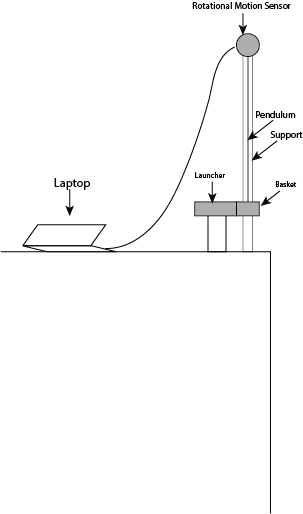
\includegraphics[height=0.85\textheight]{Pendulum Setup.png}
            \caption{Figure 1. Ballistic Pendulum Setup}
        \end{figure}
        \begin{figure}[H]
            \centering
            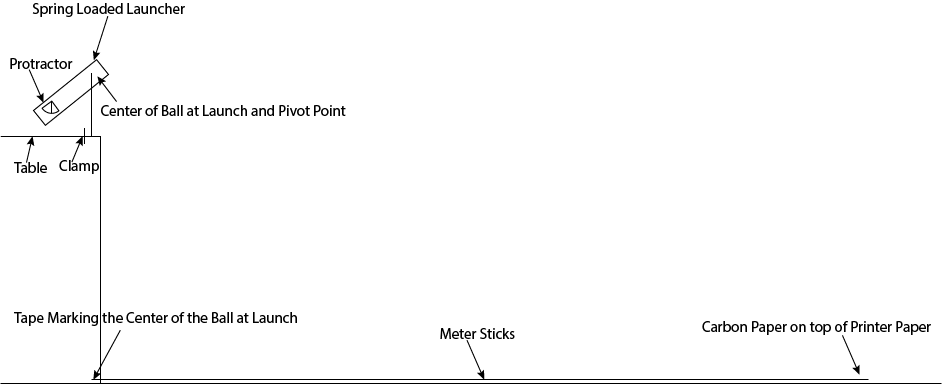
\includegraphics[width=\textwidth]{zla setup.png}
            \caption{Figure 2. Zero Launch Angle Shot Setup}
        \end{figure}
    \section{Data}
        \begin{center}
            \begin{tabular}{c|cc}
                Trial & \(\theta_{\mathrm{max}} ~( \degree )\) & \(r\) (m)\\
                \hline
                1 & 42.48 & 0.3628\\
                2 & 41.67 & 0.3659\\
                3 & 41.67 & 0.3690\\
                4 & 41.31 & 0.3680\\
                \hline
                \(\overline{x}\) & 41.81 & 0.3664\\
                \(\sigma_x\) & 0.49 & 0.0027
            \end{tabular}\\
            Table 1. Angle for maximum vertical displacement and distance from axis of rotation to center of mass.\\
            \begin{tabular}{c|cc}
                Trial & \(m_p\) (kg) & \(m_b\) (kg)\\
                \hline
                1 & 0.16915 & 0.06587\\
                2 & 0.16911 & 0.06595\\
                3 & 0.16900 & 0.06595\\
                4 & 0.16920 & 0.06594\\
                \hline
                \(\overline{x}\) & 0.16912 & 0.06593\\
                \(\sigma_x\) & 8.5x10\(^{-5}\) & 3.9x10\(^{-5}\)\\
            \end{tabular}\\
            Table 2. Masses of the pendulum and ball.\\
            \begin{tabular}{c|cc}
                Trial & \(y_0\) (m) & \(R\) (m)\\
                \hline
                1 & 1.1605 & 2.2993\\
                2 & 1.1625 & 2.3106\\
                3 & 1.1617 & 2.3170\\
                \hline
                \(\overline{x}\) & 1.6129 & 0.0090\\
                \(\sigma_x\) & 3.5x10\(^{-4}\) & 2.3090
            \end{tabular}\\
            Table 3. Zero launch angle shot.\\
        \end{center}
        \begin{figure}[H]
            \centering
            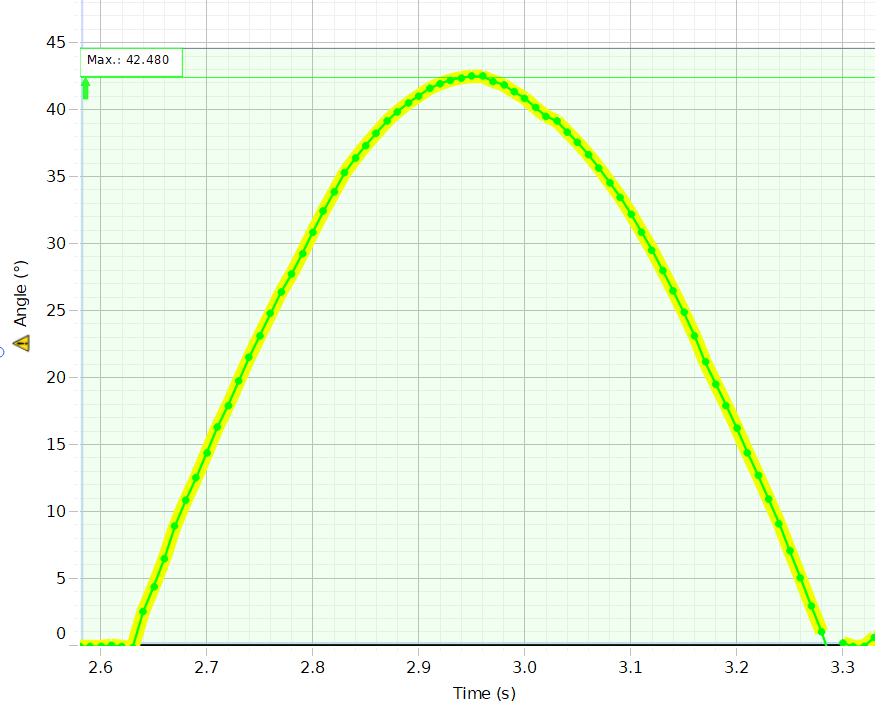
\includegraphics[width=\textwidth]{thetamax.png}
            \caption{Plot of \(\theta\) vs Time to Determine \(\theta_{\mathrm{max}}\)}
        \end{figure}
    \section{Calculations}
        \begin{alignat*}{3}
            (1)~ 
            && M & = m_b + m_p\\
            &&p_0 &= m_bv_0\\
            &&p_1 &= Mv_1\\
            &&p_1 &= p_0\\
            &&m_b v_0 &= Mv_1\\
            &&U_2 &= Mgh\\
            &&K_1 &= \frac{1}{2}Mv_1^2\\
            &&U_2 &= K_1\\
            &&\frac{1}{2}Mv_1^2 &= Mgh\\
            &&v_1 &= \sqrt{2gh}\\
            &&\frac{m_bv_0}{M} &= v_1\\
            &&\frac{m_bv_0}{M} &= \sqrt{2gh}\\
            &&v_0 &= \frac{M}{m_b}\sqrt{2gh}\\
            &&v_0 &= (1+\frac{m_p}{m_b})\sqrt{2gh}\\
            &&r &= x + h\\
            &&x &= r\cos(\theta_{\mathrm{max}})\\
            &&r &=r\cos(\theta_{\mathrm{max}}) + h\\
            &&h &=r(1-\cos(\theta_{\mathrm{max}}))\\
            &&v_0 &= (1+\frac{m_p}{m_b})\sqrt{2gr(1-\cos(\theta_{\mathrm{max}}))}\\
            (2)~
            &&\frac{\sigma_{m_b}}{\overline{m_b}} &= 0.0586\%\\
            &&\frac{\sigma_{m_p}}{\overline{m_p}} &= 0.0503\%\\
            &&\frac{\sigma_r}{\overline{r}} &= 0.737\%\\
            &&\frac{\sigma_{\theta_{\mathrm{max}}}}{\overline{\theta_{\mathrm{max}}}} &= 1.17\%\\
            (3)~
            &&v_0 & = (1+\frac{0.16912~\mathrm{kg}}{0.06593~\mathrm{kg}})\sqrt{2\cdot 9.8~ \mathrm{m/s}^2\cdot 0.3664~\mathrm{m}\cdot(1-\cos(41.81\degree))}\\
            &&&= 4.821~\mathrm{m/s}\\
            (4)~
            &&v_{0r} &= (1+\frac{0.16912~\mathrm{kg}}{0.06593~\mathrm{kg}})\sqrt{2\cdot 9.8~ \mathrm{m/s}^2\cdot (0.3664+0.0027)~\mathrm{m}\cdot(1-\cos(41.81\degree))}\\
            &&&=4.839~\mathrm{m/s}\\
            &&v_\theta &= (1+\frac{0.16912~\mathrm{kg}}{0.06593~\mathrm{kg}})\sqrt{2\cdot 9.8~ \mathrm{m/s}^2\cdot 0.3664~\mathrm{m}\cdot(1-\cos((41.81+0.49)\degree)}\\
            &&&= 4.875~\mathrm{m/s}\\
            &&\sigma_{v_0} &= \sqrt{(4.821~\mathrm{m/s}-4.875~\mathrm{m/s})^2+(4.821~\mathrm{m/s}-4.839~\mathrm{m/s})^2}\\
            &&&=0.057~\mathrm{m/s}\\
            (5)~
            &&v_0 &= R\sqrt{\frac{g}{2y_0}}\\
            &&&= 2.3090~\mathrm{m} \cdot \sqrt{\frac{9.8~\mathrm{m/s^2}}{2 \cdot 1.1629~\mathrm{m}}}\\
            &&&=4.739~\mathrm{m/s}\\
            (6)~
            &&v_R &= (2.3090 + 0.0090)~\mathrm{m} \cdot \sqrt{\frac{9.8~\mathrm{m/s^2}}{2 \cdot 1.1629~\mathrm{m}}}\\
            &&&=4.7582~\mathrm{m}\\
            &&\sigma_R &= \sqrt{(4.739~\mathrm{m}-4.7582~\mathrm{m})^2}\\
            &&&= 0.018 ~\mathrm{m}
        \end{alignat*}
    \section{Conclusion}
        The muzzle speed of the launcher was measured to be \(4.821\pm 0.057\) using the ballistic pendulum and \(4.739\pm 0.018 \) using zero launch angle shots. These two measurements are approximately within a standard deviation of each other and so it is reasonable to say that they are fairly accurate. Systematic error may have arisen from the neglect of gravity when using conservation of momentum to find the initial speed from the speed at the end of the collision and the neglect of air resistance entirely. Random error may have arisen from imperfection in how the shot was lined up with the basket, the pendulum not being perfectly still when the shot was taken, or from shaking of the launcher induced by pulling on the launcher to un-latch the spring and the force of the spring itself.
\end{document}